\documentclass[a4paper,11pt]{article}

\usepackage{graphicx}
\usepackage[sort&compress]{natbib}
\usepackage{pdfpages}
\usepackage{amsmath}
\usepackage{breqn}
\usepackage{amssymb}
\usepackage{float}
\usepackage{listings}
\usepackage[a4paper]{geometry}
\usepackage{hhline}
\usepackage{makecell}
\usepackage{amsthm}
\usepackage{caption}
\usepackage{subcaption}
\usepackage{hyperref}

\begin{document}

\theoremstyle{plain}
\newtheorem{thm}{Theorem}{}

\theoremstyle{definition}
\newtheorem{defn}[thm]{Definition}

\renewcommand{\vec}[1]{\mathbf{#1}}

\title{Research Project Proposal - Finding Interesting Patterns in Workflow Logging Data}
\date{\today}
\author{
        Dani\"el Stekelenburg		
}
 
\maketitle

\abstract{}

\section{Introduction}
Optimizing the management of business processes becomes more and more important. Companies often use a software package which helps with collecting, storing and managing data from such processes. This category of software is called ERP, which stands for Enterprise Resource Planning. An example of ERP-software is the software-package \textit{Profit}, provided by a Dutch IT-company AFAS Software BV. For our case study, we will use the historical workflow logging data of Profit, their current product. Our goal is to find interesting patterns in such data, which leads to a better understanding of what process (sub)structures represent the behavior in workflows the best.

A technology for engineering business processes is workflow management. Although a workflow does not actually have a clear definition, we use the term \textit{workflow} to refer to an organized set of \textit{tasks} to accomplish some business process \cite{Georgakopoulos1995}. The basic idea of a workflow model is to capture dependencies between process tasks in a graph. For instance, when the graph contains a relation $A \rightarrow B$, this means that task $A$ generally precedes task $B$ in an instance of this workflow. Thus, task $B$ cannot be executed until task $A$ is finished. Workflow modeling makes the intended behavior or so-called flow of a business process clear and can be used to steer such processes into the right direction.\\
The goal of \textit{workflow mining} is to revert this process, meaning that we try to find a suitable workflow based on a given set of execution logs of a business process.

\subsection{A simple example}
To make things more concrete, let us use a graph-like structure to represent a workflow. See Figure \ref{figure:example_workflow} for a simple example. The workflow shows the process of buying additional leave, and consists of a set of tasks and a set of actions. One task is the starting point - in this case \textit{Buying additional leave} - and one action is the ending point (the rightmost \textit{Accept}). For every task, I added which person needs to complete that task in order for the workflow to progress. (1) An employee fills in an application for buying additional leave, (2) his manager needs to approve the request and (3) the administrator also needs to approve this. 

\begin{figure}[H]
\centering
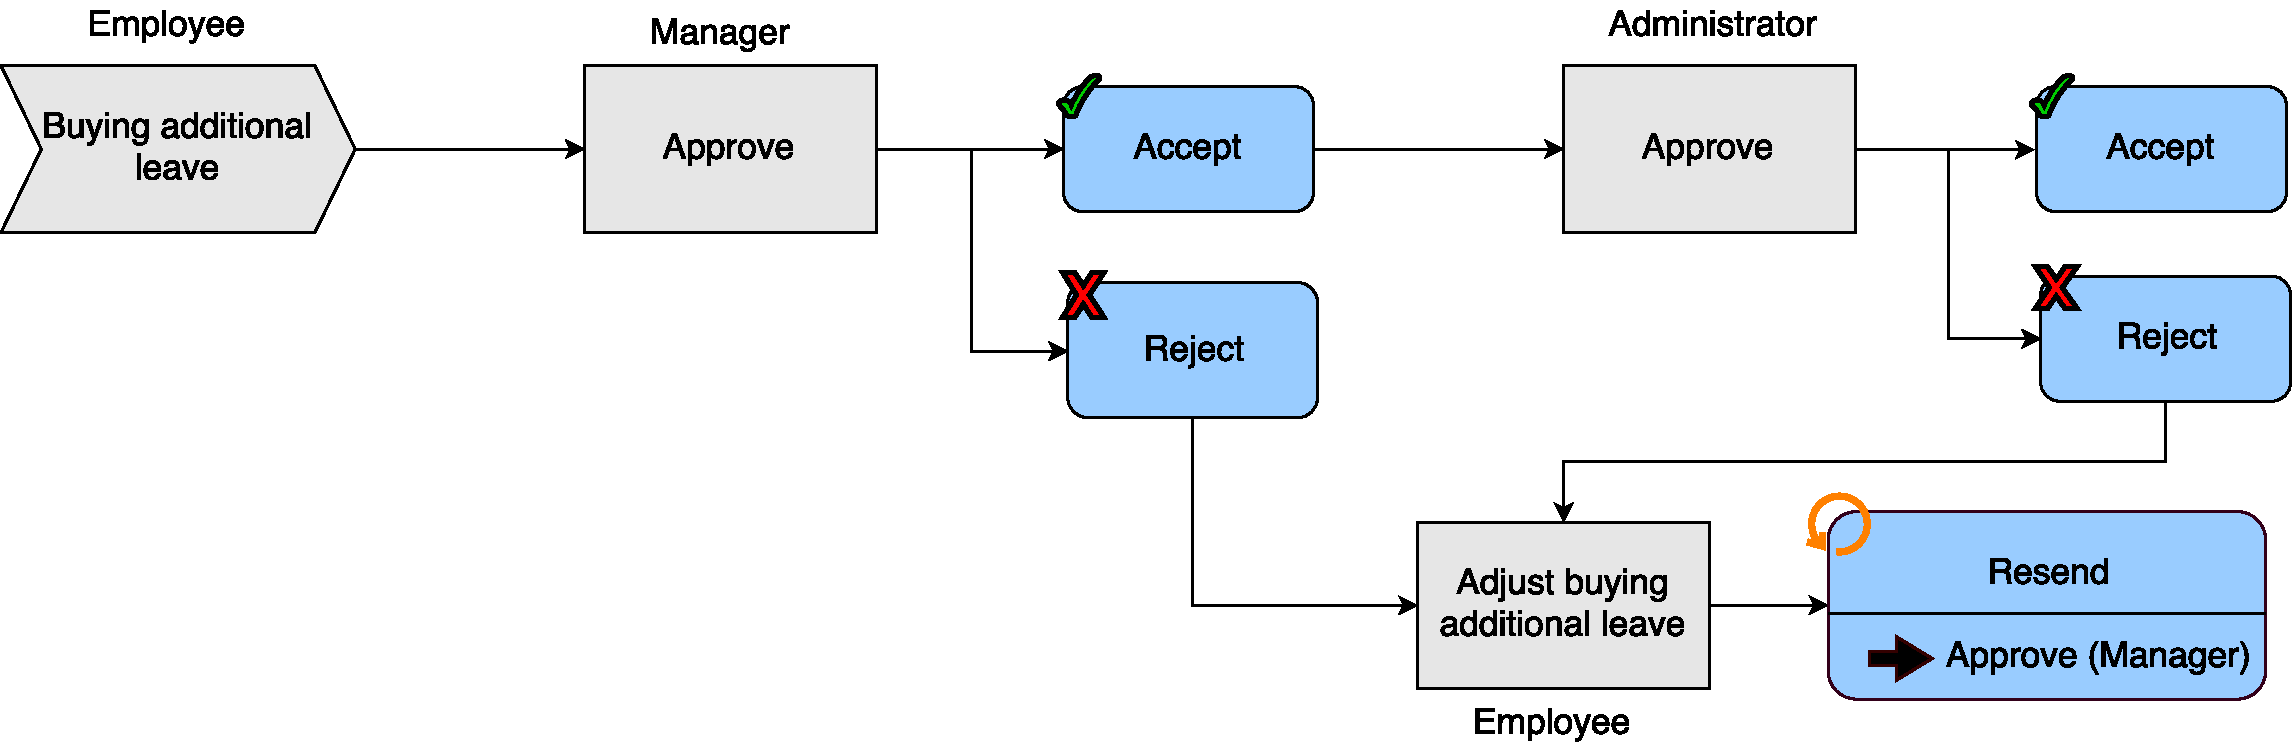
\includegraphics[width=\linewidth]{Example_Workflow.pdf}
\caption{Example workflow, representing the process of buying additional leave. Gray nodes are tasks, whereas blue nodes are actions. The dotted squares represent occurrences of the Approval pattern.}
\label{figure:example_workflow}
\end{figure}

In case one of the two approvers does not agree with the request, the employee needs to adjust his request. Note that the action \textit{Resend} refers to the task \textit{Approve}. This means that this action leads to the task \textit{Approve} (another way to show this functionality would be to simply add an arrow from \textit{Resend} to the leftmost \textit{Approve}). Finally, the workflow is completed when the rightmost \textit{Accept} action is executed.\\
Besides tasks and actions, there are workflow patterns. According to \cite{Riehle1996}, a pattern \textit{“is the abstraction from a concrete form which keeps recurring in specific nonarbitrary contexts”}. In other words, a pattern is an abstraction of a concrete set of tasks of actions and is independent of the workflow language used. An example is the or-split workflow pattern, which is visible in Figure \ref{figure:example_workflow}. Since the task \textit{Approve} has two actions and you may only choose one, you can see this structure as an OR-split.\\
The problem we try to solve, is to find certain patterns within such a workflow. However, we look beyond the purely syntactic scope of patterns and try to include the semantics or contextual meaning of a pattern. To give an example, we can say that the workflow in Figure \ref{figure:example_workflow} contains a pattern which we call the \textit{Approval pattern} ("accordeer patroon" in Dutch). In short, this pattern exists of a task which represents the decision whether some change in the system gets accepted or not. As you can see, such a decision occurs two times in the workflow: the manager needs to approve the request and also the administrator needs to approve this (indicated as the dotted areas in Figure \ref{figure:example_workflow}). So when we try to find occurrences of the approving pattern, we would like to see these two parts of the workflow in the result of our query.

\subsection{Purpose of this study}
As a business company, you often can use workflows provided with your ERP-software package or create your own workflow. Provided workflow templates are in general workflows which represent very common business processes and most companies would like to use them. When you would like to have a workflow for a very specific process, you might have to assemble your own workflow structure. However, setting up such a workflow can become quite complex which can easily lead to errors in the model defined. Especially when you have to consider multiple different use cases.\\
To remove the burden of giving the user the option to define a workflow on such a low level by itself, we want to discover workflow patterns on a higher level. This way, we can abstract away from the low level representation of a workflow and use these high-level patterns to describe processes in an organization.\\
\\
In the eyes of an IT-company which develops and sells ERP-software, it is important to know which processes are most common in a company and what kind of steps are most important in workflows. Of course, having a good insight in the usage of workflows will be very helpful when you want to deliver a workflow management system. Getting a better understanding of the importance of a pattern in a workflow is the goal of this research project.

This problem basically consists of the following subproblems:
\begin{enumerate}
\item What is a pattern?
\item When are two patterns equal?
\item When is a pattern frequent?
\item How can we mine occurrences of a pattern from a collection of logging data?
\end{enumerate}
We answer these subproblems formally in the next section.

\section{Preliminaries}
Let us state some basic definitions which we use throughout this thesis.
First of all, let us give a formal description of what a workflow (pattern) is.
\begin{defn}[Workflow]
A \textit{workflow W} is a set of tasks \textit{T} and corresponding actions $A$, set up to accomplish some business process.
\end{defn}

\begin{defn}[Workflow Pattern]
A \textit{workflow pattern p} is a subset of a workflow $W$, i.e. $p \subset W, a_p \in A, t_p \in T$, such that this pattern represents a specific objective $O$.
\end{defn}
Recall the ``Approving pattern" from the example workflow in Figure \ref{figure:example_workflow}, which consists of the task \textit{Approve} and actions \{\textit{Accept, Reject}\}. The objective $O$ is in this case the \textit{approval} of something.

\begin{defn}[Workflow pattern similarity]
Two workflow patterns $p$ and $p'$ are said to be similar if they represent the same objective $O$. Thus, $p=p'$ i.f.f. $p \rightarrow O \wedge p' \rightarrow O$.
\end{defn}

\section{Workflow Event Data}
Since more than 10 years ago, workflow events are being logged in the software package Profit. These logs are essentially a table where every record represents an action on a task in a certain workflow instance. Although the logs contain more fields, the most relevant fields are shown in an example log in Table \ref{table:log}. The first field is the \textit{Workflow ID} and is a unique reference to a workflow model (task/action graph like in Figure \ref{figure:example_workflow}) where this event sequence is based on. Although I did not include more workflows in the example, there are many workflow models used, so this field is not trivial. By grouping on this field, you collect all event logs of that specific workflow log.

The \textit{Case ID} denotes the instance or event sequence of a given workflow. Another way to refer to an event sequence is by using a tuple $<\text{Workflow ID}, \text{Case ID}>$. The \textit{Task ID} is a key for the current task in the sequence. The \textit{Action ID} refers to the action, given a task. Note that this value is not unique in a workflow. Every task within a workflow must have at least one action, and these action ID's all start at 1. The purpose of using these id fields will become more clear when I discuss the pre-processing steps planned on this data.

Then we also have two fields \textit{Task Desciption} and \textit{Action Description} which represent the actual meaning or reasoning behind a task or action in the workflow. These descriptions are words given by the creator of the workflow. Since we are interested in the context of such tasks or actions, these fields will become crucial for determining this context.
Finally, the last two fields \textit{Start Time} and \textit{End Time} contain the time stamps of this action. When you see a workflow as a finite state machine, the moment that the current task is entered is the start time of this state, whereas the moment that the action is triggered is the end time of this state. Using this information, we can derive the order of events in a sequence.

Using this information, we can derive that the log contains two event sequences, shown in Table \ref{table:example_sequences}. 

% Please add the following required packages to your document preamble:
% \usepackage{graphicx}
\begin{table}[H]
\centering
\caption{An example workflow event log.}
\label{table:log}
\resizebox{\textwidth}{!}{%
\begin{tabular}{|l|l|l|l|l|l|l|l|}
\hline
Workflow ID & Case ID & Task ID & Task Description               & Action ID & Action Description & Start Time     & End Time       \\
\hline
1           & 82      & 1       & Approve order (Manager)        & 1         & Accept             & 2-1-2017 09:10 & 2-1-2017 11:15 \\
1           & 82      & 2       & Approve order (Administrator)  & 1         & Accept             & 2-1-2017 11:15 & 2-1-2017 11:42 \\
1           & 83      & 1       & Approve order (Manager)        & 2         & Reject             & 2-3-2017 08:36 & 2-3-2017 08:49 \\
1           & 83      & 3       & Adjust buying additional leave & 1         & Resend             & 2-3-2017 08:49 & 2-3-2017 09:11 \\
1           & 83      & 1       & Approve order (Manager)        & 1         & Accept             & 2-3-2017 09:11 & 2-3-2017 09:17 \\
1           & 83      & 2       & Approve order (Administrator)  & 2         & Reject             & 2-3-2017 09:17 & 2-3-2017 09:33 \\
1           & 83      & 3       & Adjust buying additional leave & 1         & Resend             & 2-3-2017 09:33 & 2-3-2017 09:53 \\
1           & 83      & 1       & Approve order (Manager)        & 1         & Accept             & 2-3-2017 09:53 & 2-3-2017 10:04 \\
1           & 83      & 2       & Approve order (Administrator)  & 1         & Accept             & 2-3-2017 10:04 & 2-3-2017 10:11 \\
\hline
\end{tabular}%
}
\end{table}

% Please add the following required packages to your document preamble:
% \usepackage{graphicx}
\begin{table}[H]
\centering
\caption{Sequences of workflow with ID 1, based on the workflow log in Table \ref{table:log}.}
\label{table:example_sequences}
\resizebox{\textwidth}{!}{%
\begin{tabular}{r|l|l}
\begin{tabular}[c]{@{}l@{}}Case ID $\rightarrow$\\ Step in workflow$\downarrow$\end{tabular} & 82                                     & 83                                     \\
\hline
1                                                                  & Approve order (Manager) - Accept       & Approve order (Manager) - Reject       \\
2                                                                  & Approve order (Administrator) - Accept & Adjust request - Resend                \\
3                                                                  &                                        & Approve order (Manager) - Accept       \\
4                                                                  &                                        & Approve order (Administrator) - Reject \\
5                                                                  &                                        & Adjust request - Resend                \\
6                                                                  &                                        & Approve order (Manager) - Accept       \\
7                                                                  &                                        & Approve order (Administrator) - Accept
\end{tabular}%
}
\end{table}

Of course, we cannot start mining workflow patterns directly from workflow logs like described above. Some steps need to be made before mining techniques can be applied. Now that we have seen what kind of data we will be working with, let's discuss possible actions which translates this raw data into something we can use for mining high-level workflow patterns.

\subsection{Pre-processing phase}
First of all, the log needs to be ordered. This ordering is done in the following way

\begin{equation}
\text{Workflow ID} \downarrow \quad \text{Case ID} \downarrow \quad \text{Start Time} \downarrow \quad \text{End Time} \downarrow
\end{equation}

Applying this ordering results in a table where the records are chronologically ordered. This means that consecutive events within an instance of an workflow are placed together and their order goes from first to last event. 

Important to note is that we do not know the workflow model beforehand. Although the example log from Table \ref{table:log} is based on the model in Figure \ref{figure:example_workflow}, in general we do not have access to the corresponding model. Why you might ask? Well, Profit itself only contains templates and basic workflows, but many processes use a workflow which is further customized. Customers can change a standard workflow to their own wishes or make a complete new workflow model to fulfill their wishes. Since the configuration of workflows can be done by customer, these versions are not stored in one central unit, but every environment keeps track of the workflows it uses. Thus, we need to find a way to derive the workflow model from the event logs we obtained. More on this is explained later.

Another issue is that different versions of a workflow can be used throughout time. This means that different descriptions for tasks/actions can be used, or tasks/actions who previously existed in the model can be removed in later versions. Unfortunately, the event logs do not refer to a specific version of a workflow model. This causes a problem when mining for relations between tasks and actions. To give an example, recall the example workflow in Figure \ref{figure:example_workflow} and suppose that, at some point in time, the description of the first task Approve gets changed to Check. The result of this change, is that all upcoming instances of the workflow use a task called ``Check", whereas we before logged ``Approve''. How do we determine that instances using ``Approve'' and instances using ``Check'' use a different workflow model? We can do this by iterating over all instances of a workflow, keeping track of a dictionary where we store the description of every task as a tuple $<\text{Task ID}, \text{Task Description}>$. By starting at the most recent instance, you collect the latest workflow model. When an instance uses a different description for a task, given the Task ID, then you know that its workflow version is different. The same goes for changed actions in a model. This way, we can recognize which instances belong to the same workflow version. This recognition is very important, since we want to derive the correct model and this can only be done when we know which event sequences are based on this model. Using logs which used a different model will of course influence our mined model in a negative way.



\section{Problem}
The challenge which we undertake in this thesis, is to reason about interesting patterns in a given collection of workflow event logs. As a case study, we use the data of the current product of our case company AFAS Software BV. Before defining \textit{interesting} in our context, we want to know the behavior of workflows and hope to find patterns which represent this behavior the best. Note that we want to look further than the syntactic value of a pattern. We try to come up with a technique such that we can also mine patterns based on their semantics, which will give us a lot more information.\\
\\
During an iterative development, including meetings with domain experts of AFAS, we try to discover workflow patterns from which AFAS knows that they exist. However, the behavior of these workflow patterns are still unknown. Thus, by mining and analyzing occurrences of such patterns, we hope to find certain properties about these patterns. Drawing conclusions about such properties are being studied by the use of hypotheses testing. Which hypotheses will be tested, differs from the current pattern that we study. The meetings with domain experts at AFAS will be crucial for this phase.\\
\\
If the analysis of the patterns known by AFAS is completely finished, we will try to discover other patterns.

% ANSWER THE QUESTIONS STATED IN THE PREVIOUS SECTION

\section{Literature Study}
This section refers to previous works, presenting theories and techniques around workflows, workflow patterns and the problem of mining such structures using workflow logs which are valuable for our research.\\
\\
% Talk about process re-engineering in general and about workflows
Business process re-engineering is firstly proposed by \cite{Hammer1990} as an approach to tackle the problem of improving the quality of business processes, while reducing their cost. One of the earlier works presenting workflow management systems are \cite{EngelGLT79,Ellis1982}. The term \textit{information control net model} gets introduced by \cite{Ellis1982}, which can be seen as one of the earlier variants of workflow models. 

As I mentioned earlier, there are no real standards when it comes to the workflow paradigm \cite{VanderAalst1997}. This causes that management systems use different modeling languages, but a more important problem is the ability of verifying and analyzing workflows is often not available in such tools \cite{VanderAalst1997}. Because of this reason, \cite{VanderAalst1997} shows that a class of \textit{Petri nets} can be used as a way to represent workflows, which they call \textit{WF-nets}. Also, the correctness of WF-nets can be analyzed using the Petri net theory. 

% Talk about workflow patterns

The most common way to verify whether a workflow language is a good representation is by checking which \textit{workflow patterns} are covered by this language. A workflow pattern is described by \cite{Riehle1996} as \textit{``the abstraction from a concrete from which keeps recurring in specific nonarbitrary contexts"}, which holds that a pattern represents a certain functionality in a workflow while being dependent of the modeling language. Many \cite{VanderAalst2003Patterns,Dijkstra2003ControlPatterns,Russell2004DataPatterns,Russell2005ResourcePatterns,Russell2006ExceptionPatterns} describe workflow patterns providing functional requirements for workflow model languages. As stated in \cite{VanderAalst2003Patterns,Dijkstra2003ControlPatterns,Russell2004DataPatterns,Russell2005ResourcePatterns,Russell2006ExceptionPatterns}, a workflow pattern is defined by (1) a set of conditions which must be satisfied to be applicable, (2) examples of business situations where this pattern should be applied, (3) a problem description stating why applying this pattern is not trivial and (4) implementation solutions.

% Talk about workflow mining
Whereas the notion of process mining emerged within the last two decades \cite{VanderAalst2003}, the concept of workflow mining is first introduced by \cite{Agrawal1998}, where an algorithm is presented which has a set of unstructured executions of a business process as input, and outputs a minimal dependency graph representing the control flow of this business process. Furthermore, they discuss ways to cope with cycles in the graph and noise in event logs (missing executions of tasks or wrongly inserted tasks in a log). Others heuristic approaches for noise and incomplete logs are presented in \cite{Maruster2002,Weijters2001,Weijters}. The heuristic approach \cite{Weijters2001,Weijters} is a combination of the following steps: (1) constructing a dependency/frequency table, (2) mining basic dependency relations out of this table and (3) creating a workflow based on the relations found. Besides using these steps, \cite{Maruster2002} presents a logistic regression model to learn when two events are direct dependencies of one another. 

\cite{VanDerAalst2002} states that it is impossible to mine every possible WF-net. They name this challenge being the \textit{rediscovery problem}: \textit{``Find a mining algorithm able to rediscover a large class of sound WF-nets on the basis of complete workflow logs."}\cite{VanDerAalst2002}. An algorithm which can successfully mine a large class of WF-nets is the $\alpha$-algorithm \cite{VanderAalst2003,VanDerAalst2002,VanderAalst2002TimedLogs}, which assumes that the given workflow log is complete (this means that every possible execution path of the business process at hand must be present in the log). Although this completeness requirement is easy to satisfy for a simple workflow, larger workflows will have more trouble. For instance, a workflow having 10 tasks which can be executed in parallel results in $10!=3628800$ possible execution sequences. As you can tell, there is a rather small chance that every possible sequence is covered in a corresponding workflow log. Besides, the $\alpha$-algorithm did have issues with loops and self-loops. Multiple extensions on the $alpha$-algorithm have been developed. like \cite{A+-algorithm2004} which could deal with such short loops, and \cite{VanderAalst2002TimedLogs} which applies the algorithm on timed logs. Timestamps in such logs can be used to study the performance and bottlenecks of tasks in a process.\\
\\

% Talk about event logging formats

% Talk about sequential pattern mining

% Talk about word2vec
When we search for research done on determining semantic meanings of words, we see that this field has attracted a lot attention in the last few years. Especially the word2vec model \cite{Mikolov2013a,Mikolov2013b} is a popular technique. This technique results in a vector space representation of words which carries semantic meanings and is very useful in natural language processing tasks. This technique is explained in further detail in Section \ref{section:word2vec}.

% Talk about workflow(pattern) mining tools
A widely used tool for process mining is ProM \cite{ProM6} (at the time of writing the latest ProM version is 6.7). This open-source, extensible framework has over 600 different plug-ins, including process mining algorithms like the $\alpha$-algorithm, who add their own functionality to the complete software package. ProM gives the user lots of possibilities when it comes down to mining event logs and the user interface helps with getting a good understanding of the structure of process models. In the article \cite{WorkflowMiner2006} are rules shown which describe the sequence- fork- and join workflow patterns. Furthermore, they made a plug-in for ProM 5.2 called ``Workflow pattern miner". 

\subsection{The word2vec model}
\label{section:word2vec}
The model is proposed in 2013 by \cite{Mikolov2013a,Mikolov2013b}. The earlier work of Mikolov et al. \cite{Mikolov2013a} explains the use of a continuous-bag-of-words model (CBOW). A bag-of-words model translates a given document as a bag of words. Since word2vec uses the notion of neural networks, let me explain this concept shortly. 

\subsubsection{Neural Networks}
An artificial neural network is based on a biological phenomenom, the human brain. Like a human brain, a neural network exists of neurons. Depending on the given information, i.e. input values, the neurons give a certain output. The input values and their weights can also be represented as vectors $\vec{x}$ and $\vec{w}$. For a more graphical example, see Figure \ref{figure:neuron}.

The input of a neuron is determined by computing average of the sum over the input values and their weights, defined as

\begin{equation}
u = \sum_{i=0}^{K}w_i x_i = \vec{w}^T \vec{x}.
\end{equation}

A neuron uses a function $f(u)$ to determine its output value. For instance, you can use a simple function like the binary threshold-function:

\begin{equation}
f(u) = \begin{cases}
1 & \vec{w}^T \vec{x} \geq \theta \\
0 & \text{otherwise}
\end{cases}
\end{equation}
Using this function, a neuron results in either a 1 or a 0. However, there are also more complex functions from which the number of possible output values is much higher, resulting in a more detailed network. But the important thing to know is, that a layer of neurons influence the next layer etc. Eventually, in the output layer, the neuron with the highest value is the classified answer of the network.

Neurons have three different types, input, hidden and output. Figure \ref{figure:neuralnetwork} presents a multi-layered neural network (note the three layers). Neurons in the input layer already have a certain value, whereas the hidden needs to compute its output values for every neuron in the next layer. Ultimately, the output layer consists of neurons representing the possible answers you are looking for. 

\begin{figure}[h]
\begin{subfigure}{.5\textwidth}
  \centering
  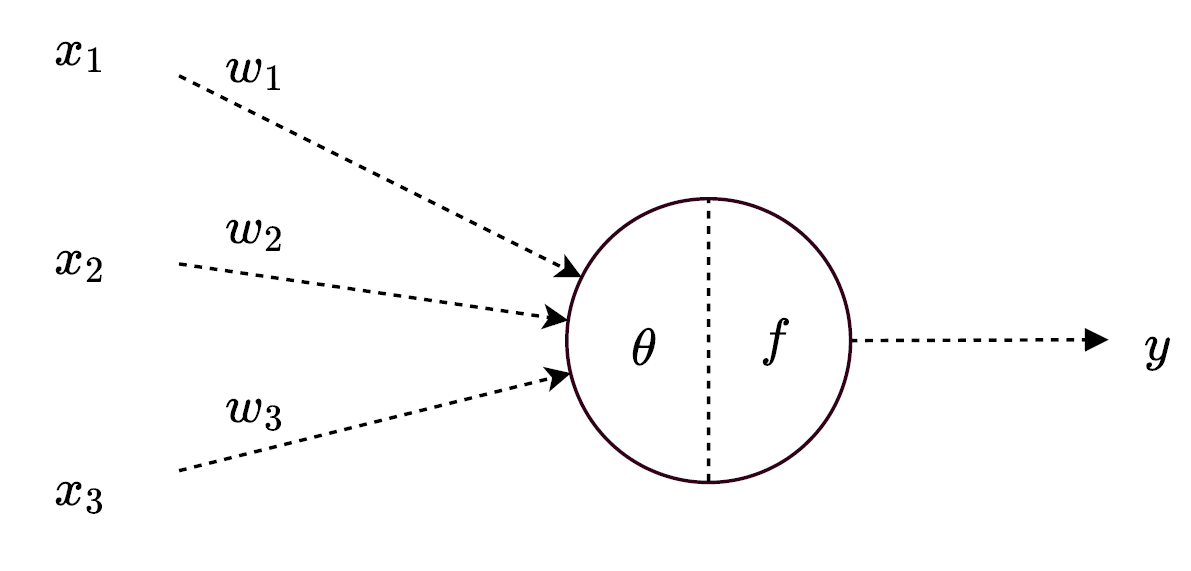
\includegraphics[width=.8\linewidth]{Neuron.png}
  \caption{A neuron.}
  \label{figure:neuron}
\end{subfigure}%
\begin{subfigure}{.6\textwidth}
  \centering
  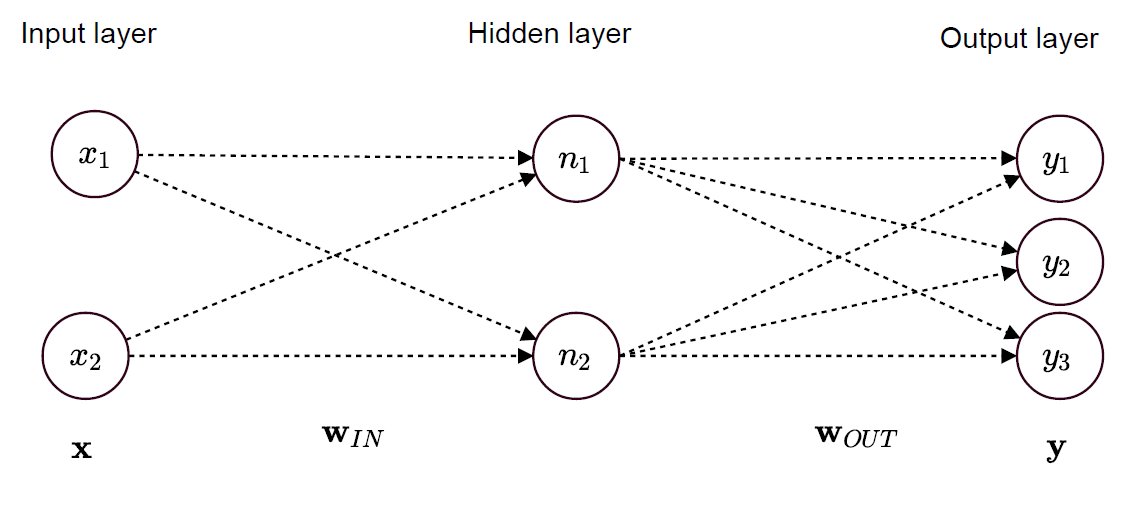
\includegraphics[width=.9\linewidth]{NeuralNetworkExample.png}
  \caption{Example of a neural network.}
  \label{figure:neuralnetwork}
\end{subfigure}
\caption{On the left, see the basic environment of a neuron. On the right, a multi-layered neural network is shown.}
\label{figure:NeuralNetworks}
\end{figure}

\subsubsection{Continuous Bag-of-Words Model}
The Continuous bag-of-words model \cite{Mikolov2013a} is the first part of the word2vec technique. This model uses context words as its input and, using a neural network, outputs the target word for which the model thinks is the most likely word with the context words as its surrounding. The simplest version of this model is a model which uses one context word, as shown in Figure \ref{figure:one-context-word}. Here, the vector $\vec{x}$ is a one-hot vector, meaning that it only contains a $1$ once and the rest of the $V$ positions are $0$'s. The size $V$ depends on the number of words used in the dictionary, and every word has a different vector $\vec{x}$.

The weights are represented by the matrices $\vec{W}_{V \times N}$ and $\vec{W'}_{N \times V}$, where every row $i$ in $\vec{W}_{V \times N}$ represents the weights vector $\vec{w}^T_i$ (with length $N$) for a context word. Thus, given a context word $w_A$, where $x = [0\ldots,0,1,0\ldots0]^T$ assuming $x_k=1$ and $x_k'=0$ for $x_k' \not= x_k$, the hidden layer will become $\vec{h}$ like,

\begin{equation}
\vec{h} = \vec{W}^T\vec{x} = \vec{W}^T_{(k,\cdot)} = \vec{v}^T_{w_k}
\end{equation}

In other words, we copy the $k$-th row of $\vec{W}$ to $\vec{h}$, which we simply call $\vec{v}^T_{w_k}$. For the output, we use matrix $\vec{W'}_{N \times V}$, which contains the weights of each $N$-sized representation of the hidden layer in order to compute the output layer. Note that the output layer, like the input layer, has the same number of neurons ($V$ in our case). This is quite obvious, since $V$ represents the number of words we can use and we are looking for a word. Computing this target word is done by computing a score $u_j$ for each possible word, like
\begin{equation}
u_j = \vec{v'}_{w_j}^T \vec{h},
\end{equation}
where $\vec{v'}_{w_j}^T$ is the $j$-th column in the matrix $\vec{W'}$. After every $u_j$ for every $j \in [1-V]$ are computed, the value for each value $y_j$ $\vec{y}$ is determined using a softmax function for normalization \cite{bishop2007pattern}:

\begin{equation}
y_j = p(w_j|w_A) = \dfrac{\exp(u_j)}{\sum_{j'=1}^V \exp(u_j')}.
\end{equation}
Here, $p(w_j|w_A)$ stands for the probability of the word $w_j$ being the target word, considering the context word $w_A$. Eventually, the highest value $y_j$ is the predicted answer of your query. The goal of training this model is to maximize the value $y_j$ for the label $w_O$, which we want to predict. The loss function $E=-log \textit{p}(w_O|w_I)$ represents the error made by the model (we try to minimize $E$). Having a perfect prediction results in $E=0$. Updating this model is done using this loss function.

\begin{figure}[H]
\centering
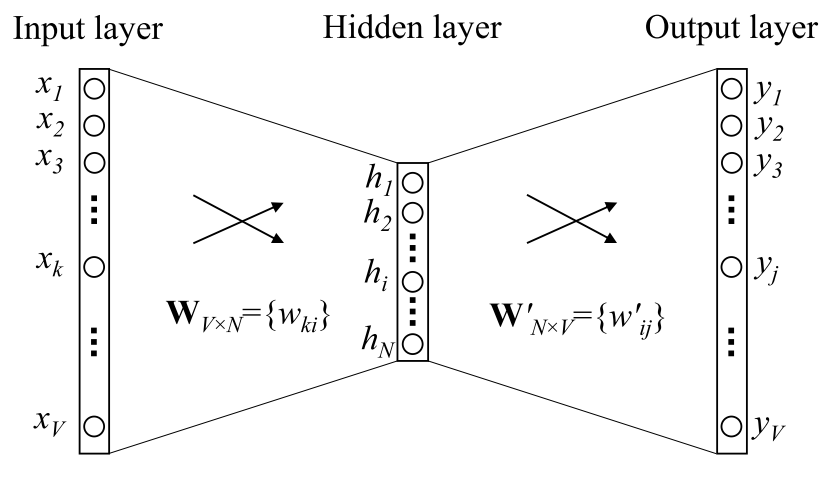
\includegraphics[width=.7\linewidth]{one-context-word.png}
\caption{CBOW model which uses only one context word as input. Source: \cite{Rong2014word2vec}}
\label{figure:one-context-word}
\end{figure}

% Explain updating the weights...

\subsubsection{Skip-gram Model}
Whereas the context words are the input of the CBOW model, the Skip-gram model \cite{Mikolov2013b} uses the target word as its input and gives the context words as output. Simply put, the skip-gram model works the other way around.

\begin{figure}[H]
\centering
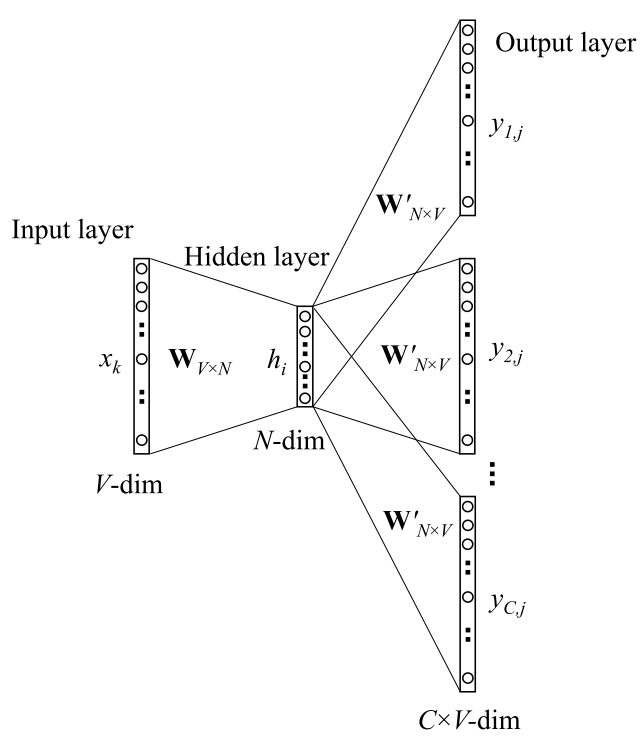
\includegraphics[width=.6\linewidth]{skip_gram.png}
\caption{The skip-gram model. Source: \cite{Rong2014word2vec}}
\label{figure:skip-gram}
\end{figure}


\section{Project Planning}
The first step in this case study is applying pre-processing steps on the available data. This means that we want the available workflow event data to be structured in such a way, that we can apply existing workflow mining algorithms on it to discover causal relations between tasks in a workflow. This phase not only consists of filtering noise or sorting/grouping the data in a certain way, but the challenge of determining which tasks or actions mean the same thing will also be tackled. Solving this problem is done by capturing the semantics of tasks and actions of a workflow. In order to achieve this, we will use the descriptions of tasks and actions. Using word2vec \cite{Mikolov2013a,Mikolov2013b}, we can represent such descriptions into a vector space model and compute the similarity between these descriptions. Based on a certain threshold value $\pi$, we determine when descriptions are said to be similar. The exact value of $\pi$ needs to be determined based on some different performance tests and will most likely differ per workflow pattern being studied.
\\
After the vector space model is trained on the descriptions of the available workflow logging data, we can start with the actual mining phase. During this phase, we will try to find occurrences of a given workflow pattern. However, this can only be done when we have structured a workflow event log into a workflow model. When we have obtained the corresponding workflow model, we can properly search for the pattern we are interested in. 

\bibliographystyle{unsrt}
\bibliography{sources}

\end{document}